% -----------------------------------------------------------------
% Document class: Article
\documentclass[ a4paper, twoside, 11pt]{article}
\usepackage{../../macros-general}
\usepackage{../../macros-article}
% Number of the handout, quiz, exam, etc.
\newcommand{\numero}{02}
\setcounter{numero}{\numero}

% -----------------------------------------------------------------
\begin{document}
\allowdisplaybreaks

\begin{center}
\Large Sistemas de Control (EYAG-1005): Evaluaci\'on \numero \\[1ex]
\small \textbf{Semestre:} 2017-2018 T\'ermino I \qquad
\textbf{Instructor:} Luis Reyes, Jonathan Le\'on
\end{center}
\halfskip

\fbox{

\begin{minipage}[b][\height][t]{\textwidth}
\vspace{0.2 cm}

\begin{center}
\textbf{COMPROMISO DE HONOR}
\end{center}
\vspace{0.4 cm}

\scriptsize
{
Yo, \rule{60mm}{.1pt} al firmar este compromiso, reconozco que la presente lecci\'on est\'a dise\~nada para ser resuelta de manera individual, que puedo usar un l\'apiz o pluma y una calculadora cient\'ifica, \linebreak que solo puedo comunicarme con la persona responsable de la recepci\'on de la lecci\'on, y que cualquier instrumento de comunicaci\'on que hubiere tra\'ido debo apagarlo. Tambi\'en estoy conciente que no debo consultar libros, notas, \linebreak ni materiales did\'acticos adicionales a los que el instructor entregue durante la lecci\'on o autorice a utilizar. Finalmente, me comprometo a desarrollar y presentar mis respuestas de manera clara y ordenada. \\

Firmo al pie del presente compromiso como constancia de haberlo le\'ido y aceptado. 
\vspace{0.4 cm}

Firma: \rule{60mm}{.1pt} \qquad N\'umero de matr\'icula: \rule{40mm}{.1pt} \hspace{0.5cm} \\[-0.8ex]
}

\end{minipage}

}

\vspace{\baselineskip}



% =============================================
\begin{problem} El siguiente Diagrama de Bode muestra la respuesta de la frecuencia de un sistema de segundo orden sub-amortiguado. 

\begin{figure}[htb]
\centering
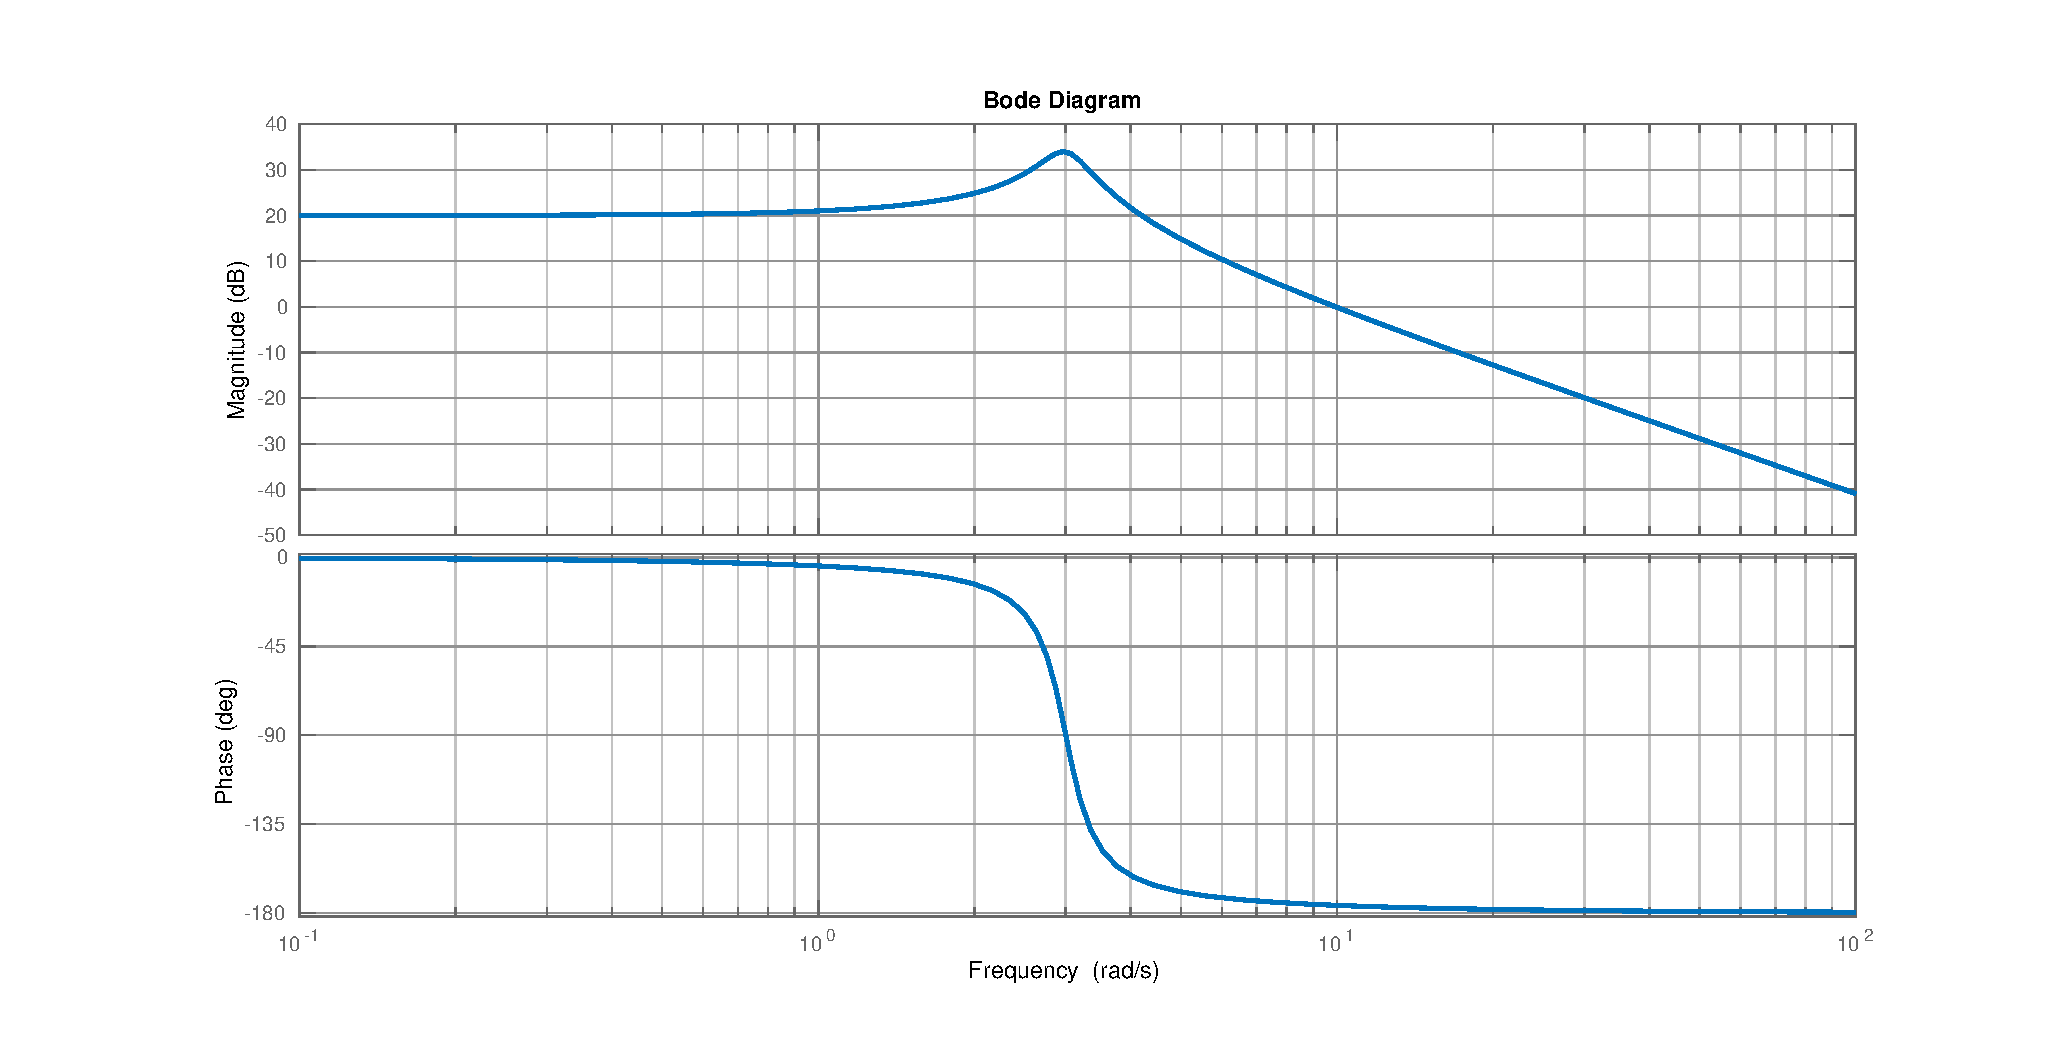
\includegraphics[width=\textwidth]{prob_bode-identificacion.eps}
\end{figure}

Complete las siguientes actividades: 
\begin{itemize}
\item \textbf{[2 Puntos]} Determine la veracidad o falsedad del siguiente enunciado: El margen de ganancia es no mayor a 15 decibeles, \ie $G_M \leq 15 \text{ dB}$. 
\item \textbf{[2 Puntos]} Determine la veracidad o falsedad del siguiente enunciado: El margen de fase es no menor de 40\deg, \ie $\phi_M \geq 40\deg \text{ dB}$. 
\item \textbf{[2 Puntos]} Determine la veracidad o falsedad del siguiente enunciado: El ancho de banda del sistema es no mayor a 4 rad/s, \ie $\omega_{BW} \leq 4$ rad/s. 
\item \textbf{[4 Puntos]} Encuentre la funci\'on de transferencia del sistema. 
\end{itemize}

\end{problem}
\vspace{\baselineskip}

% =============================================
\begin{problem}
\textbf{[10 Puntos]} Considere el siguiente compensador de atraso de fase: 
\[
G_C(s) \; = \; K \, \frac{(s+z)}{(s+p)} \, ,
\]
Encuentre valores para los par\'ametros $K$, $z$ y $p$ de tal manera que su as\'intota de baja frequencia sea de $+30$ dB, su as\'intota de alta frecuencia sea de $-10$ dB, y su fase sea de $-45\deg$ cuando su frecuencia es de 10 rad/s. 

\emph{Sugerencia:} Para escribir la ecuaci\'on asociada con el \'ultimo requerimiento recuerde que cuando la fase es de $-45\deg$ la parte real de $G( j \omega )$ es igual al negativo de su parte imaginaria. 

\end{problem}
\vspace{\baselineskip}

% =============================================
\begin{problem} \textbf{[10 Puntos]} Construya un modelo de espacio de estados que represente al mecanismo mostrado en la figura de abajo suponiendo que las salidas son las posiciones de los bloques de masa. 

\begin{figure}[htb]
\centering
\includegraphics[width=0.68\textwidth]{prob_espacio-estados.jpg}
\end{figure}

\end{problem}
\vspace{\baselineskip}

% =============================================
\begin{problem}
\textbf{[10 Puntos]} Para el siguiente modelo de espacio de estados encuentre la funci\'on de transferencia equivalente. 
\begin{align*}
\vec{\dot{x}}(t) \; & = \; 
\left[ \begin{array}{cc}
-1 & +4 \\ -4 & -1
\end{array} \right] \vec{x}(t) + 
\left[ \begin{array}{c}
+2 \\ -1
\end{array} \right] \vec{u}(t) \\[2ex]
\vec{y}(t) \; & = \; 
\left[ \begin{array}{cc}
1 & 1
\end{array} \right] \vec{x}(t)
\end{align*}

\end{problem}
\vspace{\baselineskip}

\end{document}

% =============================================
\begin{problem}
\textbf{[X Puntos]} Bosqueje el Diagrama de Bode para la siguiente planta: 
\[
G(s) \; = \; \frac{10 \, (s+144)^2}{s^2 + 0.6s + 9}
\]

\end{problem}
\vspace{\baselineskip}
